\documentclass{article}
\usepackage[utf8]{inputenc}
\usepackage{graphicx}
\usepackage{hyperref}
\usepackage{subcaption}
\usepackage{amsmath}
%\usepackage{multirow}
%\usepackage{multicol}
\title{DPhil: Transfer of Status Literature Review}
\author{Shaan Desai }
\usepackage[parfill]{parskip}

\begin{document}

% Title page is created here
\maketitle
\bibliographystyle{abbrv}

\tableofcontents
\section{Introduction}

The past decade has seen an immense dedication to research in Artificial Intelligence, most notably in Deep Neural Networks (DNNs). DNNs have been used across a whole host of domains including image classification, machine translation and time-series forecasting. Despite these grand successes, DNNs have numerous limitations. In particular, DNNs are black boxes meaning they aren't interpretable, they require many datapoints ($>5000$ points) to learn and are highly sensitive to hyperparameter tuning. Given such limitations, the physics community has been apprehensive about its adoption. However, over the past 2 years, significant research on inductive biases has paved a new road to embed knowledge from physics into DNNs. This prior knowledge has been shown to make DNNs more data efficient and more interpretable. In this review, we look at state-of-the-art methods at the intersection of deep networks and physics. For every method, we summarize the key tricks that drive performance and also mention possible pain points worth investigating further.


\section{Artificial Intelligence}

- Humans have long tried to understand how the mind works
- from a biological perspective it is clear that connectomics paves a pathway to understanding how we think
- With the advent of computers and 'large' processing power, many researchers began to ask whether the human mind can be replicated using a computer.
- Early work by walter and warren was the first to point out a means to build neural network logic.
- Followed by Hebbian
- Then an AI winter
- Geof Hinton backprop
- slew of advents in neural processing, convnets, rnns, graphs, tensor nets, deep RL, 
- all seeking to solve more tasks/increase generalizability.
- to date, there has been no general purpose solution (AGI) for a vast array of tasks e.g. a human can learn to create art, sit math exams, play sports, yet a robot so far can only do one of these tasks well.
- Numerous limitations in terms of processing power and memory access still exist

- Despite these limitations, neural networks have brought about significant advancements to society in robotics, self driving cars, cancer detection.

- In what follows, we outline some of the major advances, those which have been fundamental pillars to research conducted during this phd. We follow no particular order.

\section{Inductive Biases}

An inductive bias in machine learning is prior information used to guide model building. In simple linear regression, for example, we assume the distribution of the noise in our data follows a Gaussian. This is a natural inductive bias because prior to seeing any data, we have assumed our noise model follows this form. In neural networks, architectures with variable depth, form and activations for example, serve as inductive biases. In essence, we encode initial assumptions about the complexity of data via inductive biases. 

A feedforward deep neural network naturally encodes 'nonlinearity' as a prior and arguably makes the least assumptions about the underlying data. Convolutional Neural Networks assume spatial representations can be captured. Recurrent Neural Networks assume temporal data as inputs. 

In what follows, we highlight some of the recent advances in inductive biases, particularly as they relate to solving problems in physics.

\subsection{Graph Neural Networks}

The state of a physical system can be represented by a graph $G = (u,V,E)$ \cite{battaglia_relational_2018}. For example, a node ($V$) can be used to represent a particle in an N-body problem. These nodes can be used to represent the core features of the particle e.g. position, momentum, mass and particle constants. Edges ($E$) can represent forces between the particles and `Globals' ($u$) can represent constants such as air density, the gravitational constant etc. We note that graphs can be fully connected or sparse, depending on the specific use case. In representing physical systems this way, we impart structure on our data which forms an important inductive bias when learning physics \cite{battaglia_interaction_2016, battaglia_relational_2018, sanchez-gonzalez_graph_2018,seo_differentiable_2019,cranmer_learning_2019, seo_physics-aware_2020, sanchez-gonzalez_learning_2020,lamb_graph_2020,cranmer_lagrangian_2020}. Representations of this form allow us to carry out learning in multiple complex domains because such graphs can be input to Graph Neural Networks which can be used to update the graph attributes. In addition, graphs allow for increased interpretability \cite{battaglia_relational_2018}.

Some major applications include:
\begin{itemize}
\item Interaction-physics based problems naturally benefit from graphs \cite{battaglia_relational_2018}. 
\item We see that graph networks trained to learn Hamiltonians achieve great results in rolling out trajectories of N-body systems \cite{sanchez-gonzalez_hamiltonian_2019}. 
\item Graphs have shown significant promise in explaining the phase transition of glassy materials \cite{bapst_unveiling_2020}. 
\item They're even shown to model complex fluid like systems from visual data \cite{sanchez-gonzalez_learning_2020}. 
\end{itemize}

Graph Neural Networks are considered to impart a relational inductive bias, as convolutional networks are considered to impart a spatial bias and recurrent networks to impart a temporal bias. 

Inspired by this work we see two major steps in moving this research forward. Firstly, their use in physics opens up a tried-and-tested pathway to solve more complex problems particularly in accounting for material interactions. As such, we see good scope to use graph networks for large interacting systems as has been shown in \cite{sanchez-gonzalez_learning_2020}. Secondly, most systems to date have looked at graphs for classical physics but literature from 2004 suggests graphs, inherent in their relational structure, can also capture Ising-like hamiltonian structure.


\subsection{Integrative Biases}

In 2018, NeuralODE brought to light a meaningful connection between residual networks and integrative steps. For example, if we use a neural network to learn a function $F$ then use a residual block to add this function multiple times, in the continuous limit, this approximates a differential equation.

Residual networks consist of a discrete set of steps:
$$ h_{t+1} = h_t + f(h_t,\theta_t) $$

which take on the form a discrete euler equation. In the continuous limit, this becomes:

$$ \frac{dh(t)}{dt} = f(h(t),t,\theta) $$

We can therefore parametrize any differential equation as a neural network and integrate it as long as we know its initial condition and final time step evaluation. However, one of the challenges of passing a neural network output to an integrator is the fact that the integrator induces additional operations on the weights. Neural ODEs allow us to integrate this neural network with constant memory cost \cite{chen_neural_2018}.

The integrative bias here is used in numerous systems aimed at learning continuous time dynamics. In many settings a one-step integration is applied. For this, we do not need to use any complex ODESolver. Instead, a simple 'manual' integration is used. There are indeed settings where a multi-step integration is used, such as in \cite{zhong_symplectic_2019} and in \cite{saemundsson_variational_2019}.

\subsection{Physics priors}

Broadly, the intersection of physics and AI falls into one of two domains, physics for AI or AI for physics. The former uses techniques from physics to develop and improve learning algorithms in general. The latter uses existing learning approaches (with adaptations) to predict physics, for example ML for materials. In this review, we focus our attention on the latter.

Physicists have long been interested in using learning tools to predict physics based systems. Some of these include predicting magnetic properties of 2-D materials, predicting the time evolution of N-body systems and even using AI to understand phase transitions. However, numerous challenges still remain in terms of data-efficient learning, reducing computational cost, improving predictive accuracy and learning better representations of the underlying physical process. Researchers have identified methods to address these challenges, but arguably the most promising hinges on physics-informed priors embedded in learning. It has been shown that models enriched with physically-informed priors i.e. models which consist of some knowledge about the physical system apriori, significantly outperform traditional methods in terms of data-efficiency and predictive accuracy. This has sparked a sharp interest in building both task-specific and general physics priors to improve learning. In this section, we summarize some of the core developments over time in physics informed inductive biases. 

\subsubsection{Gradient Learning}

Although most modern methods cite gradient learning by Witkoskie as one of the earliest efforts designed to improve learning of physics in neural networks, we actually find that more sophisticated approaches were developed prior to this effort.

In 1996 James Howse/NIPS presented a paper which highlights a few things on identifying dynamical systems. The paper introduces a model inspired by defining a generalized functional form for dynamical systems. Using a potential $V(x)$ we can partition an n-dimensional phase space in which the first space is normal to a level surface $V(x)=k$, and the second is tangent to $V(x)=k$. Systems which always move downhill are gradient like systems: $ \dot{x} = - P(x)\nabla_{x} V(x) $. Systems which remain at constant potential are Hamiltonian like: $\dot{x} = Q(x)\nabla_x V(x)$. The combination of the two can  be used to get total dynamics.

The entire framework is a parameter fitting one because we have a sense for the prior functional form of the dynamics.

The notion of embedding physically-informed inductive biases in neural networks can be found in numerous early work aimed at modelling materials \cite{witkoskie_neural_2005, pukrittayakamee_simultaneous_2009, smith_ani-1_2017, rupp_fast_2012, yao_tensormol-01_2018}. For example, early efforts by Witkoskie and Doren \cite{witkoskie_neural_2005} demonstrate that in contrast to directly learning a potential energy surface, the inclusion of gradient learning can drive a network to accurately model the forces. 

Therefore, the loss function takes the form:
$$
\Bigg\|
\begin{bmatrix}
\hat{y} \\
\hat{\dot{y}}
\end{bmatrix}
-
\begin{bmatrix}
y \\
\dot{y}
\end{bmatrix}
\Bigg\|_2^2
$$

This addition means that we can supplement the learning process with additional information and hence improve the learnt potential surface. The fundamental idea being that if we have access to supplemental data such as the gradients, but fewer data points, we might actually learn a surface with higher accuracy than if we had many data points with no gradient information. 

This result inspires us to look more closely at combining inductive biases. Namely, by adding well known priors together, we may make learning data-efficient and more accurate.

\subsubsection{Physics Informed Neural Networks}

PINNs is one of the first methods to use the backpropagation technique from neural networks to actually compute the gradients of a function with respect to the inputs of that given function. For example, given t and x, PINNs compute $u(t,x)$ through which they can compute gradients of u w.r.t. t and x. A concrete example is this differential equation:


$$ u_t + N[u] = 0$$

where N is a nonlinear differential operator and $u(t,x)$ denotes the latent hidden solution.

Using the equation we can define:

$$ f = u_t +N[u] $$

then we can, for any set (t,x), compute u(t,x) with a neural network. Using backpropagation, we can then compute partial derivatives w.r.t the input variables. The final results can thus be stored in f. A simple L2 loss to minimize the predicted u vs the ground truth u (for initial and boundary conditions) coupled with a penalization of the function f (since it should be zero) at specific collocation points results in PINNs.

PINNs are used for both data-drive solution and data-driven discovery. In other words, PINNs can be used to identify a systems governing equations or given a set of equations, be used to continuously solve the system given an initial condition and points of evaluation.





\subsubsection{Deep Lagrangian Network}

DeLAN net is the first network to use a lagrangian embedded in a neural network to learn the dynamics of a system. 

In the paper they define:
$$ L = T - V$$
and
$$ \frac{d}{dt}\frac{\partial L}{\partial \dot{q}} - \frac{\partial L}{\partial q} = \tau $$

where $\tau$ represents generalized forces.

If we are dealing with a rigid body then: $ T = \dot{q}^T M(q) \dot{q} $ where M is the inertia matrix. Replacing this equation in euler-lagrange results in:

$$ \frac{d}{dt} (M(q)\dot{q}) - \frac{\partial V}{\partial q} = 0 $$

$$ M(q)\ddot{q} = \dot{M(q)} \dot{q} + \frac{\partial V}{\partial q} $$

To get $\ddot{q}$ all we need is M and its time derivative. 

$$ p = M(q) \dot{q} $$

As a result of this framing, DeLAN net uses multiple network heads to compute individual components of the equation before combining them. 

\subsubsection{Hamiltonian Neural Networks}
\label{HNN}
ing neural networks to accurately learn classical dynamics from data  problems has been Hamiltonian Neural Networks \cite{greydanus_hamiltonian_2019}. In  demonstrated that dynamic predictions through time can be improved using Hamiltonian Neural Networks (HNNs) which endow models with a Hamiltonian constraint. The Hamiltonian is an important representation of a dynamical system because it is one of two approaches that generalizes classical mechanics. The Hamiltonian $\mathcal{H}$ is a scalar function of position $\mathbf{q} = (q_1,q_2,....,q_M)$ and momentum $\mathbf{p} = (p_1,p_2,....,p_M)$. In representing physical systems with a Hamiltonian, one can simply extract the time derivatives of the inputs by differentiating the Hamiltonian with respect to its inputs (see Eqn. \ref{eqn.hamiltonian}.)
\begin{equation}
\frac{\mathrm{d}\mathbf{q}}{\mathrm{d}t} = \frac{\partial \mathcal{H}}{\partial \mathbf{p}}, ~~~
\frac{\mathrm{d}\mathbf{p}}{\mathrm{d}t} = -\frac{\partial \mathcal{H}}{\partial \mathbf{q}}
\label{eqn.hamiltonian}
\end{equation}
As a consequence, it is noted in \cite{greydanus_hamiltonian_2019} that by accurately learning a Hamiltonian, the system's dynamics can be naturally extracted through backpropagation. This information allows us to build two 1st-order differential equations which can be used to update the state space, $(\mathbf{q},\mathbf{p})$. Equation \ref{eqn.action_int} shows this integral, in which we define the symplectic gradient $\mathbf{S}  = \left [ \frac{\partial \mathcal{H}}{\partial \mathbf{p}},-\frac{\partial \mathcal{H}}{\partial \mathbf{q}} \right ] $:
\begin{equation}
(\mathbf{q},\mathbf{p})_{t+1} = (\mathbf{q},\mathbf{p})_t + \int_t^{t+1} \mathbf{S}(\mathbf{q},\mathbf{p}) \mathrm{d}t
\label{eqn.action_int}
\end{equation}
%However, this is not the only benefit in learning a Hamiltonian. Another key attribute of the Hamiltonian is that the vector field $\mathbf{S}$ is a symplectic gradient meaning $\mathcal{H}$ remains constant as long as state vectors are integrated along $\mathbf{S}$. This result links the Hamiltonian with the total energy of the system $\mathcal{H}(\mathbf{q},\mathbf{p}) = E_{tot}$. 
It can be shown that the Hamiltonian in many systems also represents the total energy of the system. Therefore, the Hamiltonian is a powerful inductive bias that can be utilised to evolve a physical state while maintaining energy conservation.

\subsubsection{Variational Integrator Networks}

Lagrangian mechanics offers an alternative to the Hamiltonian in generalizing a dynamical system. Rather than position and momentum (canonical coordinates) defining the state space, Lagrangian mechanics is defined using a generalized coordinate state space $(\mathbf{q},\dot{\mathbf{q}})$. This is particularly useful in physical settings where the description and measurement of generalized coordinates may be easier to work with than canonical coordinates \cite{marsden_discrete_2001}. Given these coordinates, Joseph-Louis Lagrange showed that a scalar value $\mathcal{A}$, referred to as the action, can be defined as the integral of a Lagrangian, $\mathcal{L}(\mathbf{q},\dot{\mathbf{q}})$:
\begin{equation}
\mathcal{A} = \int_{t}^{t+1} \mathcal{L}(\mathbf{q},\dot{\mathbf{q}}) \mathrm{d}t
\label{eqn.action_integral}
\end{equation}
The integral can be thought as inducing multiple paths between points in state space i.e. multiple walks in the domain of $(\mathbf{q},\mathbf{\dot{q}})$. However, only one path is a stationary state of the action integral. This state lets us move from $t \rightarrow t+1$ with minimal energy. It can be shown, through variational calculus, that this stationary state must satisfy the Euler-Lagrange equation:
\begin{equation}
\frac{\mathrm{d} }{\mathrm{d}t} \left ( \frac{\partial \mathcal{L}}{\partial \dot{\mathbf{q}}} \right )= \frac{\partial \mathcal{L}}{\partial \mathbf{q}}
\label{eqn.euler_lagrange}
\end{equation}
Although complex in form, the action integral and the Euler-Lagrange equations can be discretized and collectively form the basis for variational integrators. The work in \cite{saemundsson_variational_2019} shows that, by adopting this approach, one can develop VINs which make network learning in noisy data-settings more robust. Similar to Hamiltonians, Lagrangians in classical mechanics are also connected to the kinetic energy $\mathcal{T}$ and potential energy $\mathcal{V}$ via:
\begin{equation}
\mathcal{L} = \mathcal{T}(\mathbf{q},\mathbf{\dot{q}}) - \mathcal{V} (\mathbf{q},\mathbf{\dot{q}})
\end{equation}
Furthermore, Variational Integrators are symplectic and momentum conserving \cite{lew_overview_nodate}.

\subsubsection{Symplectic ODE Net}

Symp-ODEN \cite{zhong_symplectic_2019} extends hamiltonian neural networks into the control domain. If external control is affine and influences the change in generalized momenta then:

$$ 
\begin{bmatrix}
\dot{q} \\
\dot{p}
\end{bmatrix}
= 
\begin{bmatrix}
\frac{\partial H}{\partial p} \\
-\frac{\partial H}{\partial q}
\end{bmatrix}
+
\begin{bmatrix}
0 \\
g(q)
\end{bmatrix} u
$$

If rank(g(q)) is rank(q) the system is fully actuated. For such systems, a controller $u = \beta(q) +v(p) $ can be designed to change the potential energy landscape so as to force a system toward a specific configuration.

If the hamiltonian is a newtonian then - $$ \beta(q) = g^T (gg^T)^{-1} (\partial V/\partial q - \partial V_d/\partial q) $$


\subsubsection{Symplectic Recurrent Neural Network}

Symplectic RNN \cite{chen_symplectic_2020} makes two major contributions to the physics neural network space. Firstly, they take \nameref{HNN} and convert the integration scheme from euler to a leapfrog. Secondly, they adopt a NeuralODE style integrator to integrate across multiple timesteps from an initial condition.


\subsubsection{Symbolic Pregression}

Fundamental early work aimed at devising unique ways to find regression coefficients using a supervised learning framework. Symbolic pregression combines this approach with that of the hamiltonian neural net to build an unsupervised framework for discovery of differential equations \cite{udrescu_symbolic_2020}.

\subsubsection{Deep Energy Network}

A new method is introduced to tackle the challenge of learning energy conserving physics more broadly. The method claims to be more general as it can learn from PDEs as well as ODEs, and it avoids discretisation errors that arise from using RK integrators. The method does this by a) introducing a general formalism which highlights how the rate of change of states can be cast into a matrix G times the gradient of a Hamiltonian and b) by discretising the gradient of the hamiltonian with a frechet derivative. 
\begin{equation}
 \dot{u} = G\nabla H
\end{equation}
 
The main benefit is that it can solve a broader class of problems compared to current solutions in the field by modelling an additional G matrix e.g.
Friction systems (ODE and PDE)
Discrete PDEs (PDE)
Maintains energy and mass conservation via discretisation which preserves the geometric structure (a.k.a volume preservation)
Good form for discrete auto differentiation
Great PDE dataset motivations
Can extend research to identify discrete PDEs

\subsubsection{Unsupervised Learning of Lagrangian Dynamics}

In \cite{zhong_unsupervised_2020}, the authors show that the full Lagrangian dynamics can be learned from visual data. The paper introduces a co-ordinate aware VAE to encode the latent space and then computes the derivatives of the state. The introduction of co-ordinate awareness is to ensure a bijective function. The paper shows that the motion of a pendulum can be learnt from visual data. More importantly, via energy shaping, the pendulum can be constrained into a configuration $q*$ of choice.

\subsubsection{Lagrangian Neural Networks}

The main premise of LNNs \cite{cranmer_lagrangian_2020} is to tackle the problem of dealing with coordinate spaces. Many datasets do not usually consist of  canonical position and momentum, rather they use generalized coordinates. As such, LNNs aim to tackle learning from generalized coordinates. In addition, they provide a more general framework than DeLaNs which were designed to work well with continuous control applications. The unique trick that LNNs introduce over other methods is that they do not assume any form for the lagrangian. 

In vectorized form, euler lagrange is:

\begin{equation}
\frac{d}{dt} \nabla_{\dot{q}} \mathcal{L} = \nabla_q \mathcal{L}
\label{eqn.lnn1}
\end{equation}

Using chain rule to expand the time derivative e.g. allow $\nabla_{\dot{q}}\mathcal{L}$ to be a function of $q$ and $\dot{q}$ then:

\begin{equation}
(\nabla_{\dot{q}}\nabla_{\dot{q}}^T \mathcal{L}) \ddot{q} + (\nabla_q \nabla_{\dot{q}}^T \mathcal{L})\dot{q} = \nabla_q \mathcal{L}
\end{equation}

Then, with matrix inversion, one can obtain $\ddot{q}$. 

Using this term, one can minimize the loss on the state vector $[q,\dot{q},\ddot{q}]$. The paper shows promising results on the double pendulum, relativistic particle in a uniform potential and on the wave equation. Upon inspection of the training scheme for the highly sensitive double pendulum, we do find that training times and data points are quite large, creating a space to find a more optimal learning scheme.

\subsubsection{Modeling System Dynamics with PINNs on Lagrangian Mechanics}

Unlike LNNs, this paper introduces a functional form for the Lagrangian. The Lagrangian in this paper \cite{roehrl_modeling_2020} is assumed to be $L = T -V$. In addition, they introduce non conservative forces and the final form is:

$$ M(q) \ddot{q} + C(q,\dot{q})\dot{q} + G(q) = Q^{ncons} $$

The approach taken by this paper is to feed in the respective components e.g. q,$\dot{q}$ into separate neural network heads designed to predict one of M, C and G. Using this technique, $\ddot{q}$ is backed out and then fed to an RK-4 integrator.

The approach is tethered to a more traditional way of using NNs for predictions and is one of the reasons why model performance is not as good as it can be if backpropagation was used to compute the second derivative of q. In addition, the wrong choice of integrator is a bottleneck for long range predictions in this setting.

\subsubsection{Thermal}


\subsubsection{Learning Constrained Dynamics with Gauss' Principle adhering Gaussian Processes}

The paper \cite{geist_learning_2020} introduces GP model that utilises mechanical constraints as prior knowledge for learning dynamics of systems. The GP is constrained to satisfy Gauss Principle. 

Using UKE, the acceleration of a particle can be disentangled into unconstrained acceleration, ideal part of constraint and non-ideal part of constraint.  Using this knowledge, one can feed this structural form into the mean of a GPR. The process can be used to set priors on unknown parameters. The learned model appears to capture dynamics much better than standards GPs without the underlying equation needed to be satisfied in the mean of the GP.





\subsubsection{Quantum based NNs}


\subsubsection{Holonomic constraint}



\subsubsection{SympNets}

A brand new class of methods is proposed . It avoids the need for a separable Hamiltonian and more importantly, is designed to eliminate the need for backpropagating the Hamiltonian with respect to the input. In this framework, a sequence of symplectic maps are used to transform the input into the output. The symplectic map can be split into an upper triangular matrix and lower triangular matrix with diagonals set to 1. Non-diagonal terms are parametrized by a NN and by stacking a range of symplectic maps together, one can learn dynamics better. In fact, the results show that by doing this, the learned trajectory is significantly more accurate than HNNs with symplectic integrators!

\subsubsection{Deep Hamiltonian Networks based on symplectic integrators}

This paper \cite{zhu_deep_2020} reviews the integrator of choice for hamiltonian neural networks. One of its primary objectives is to establish the difference in performance between using a symplectic vs non-symplectic integrator from a theoretical perspective. Quite evidently, using a symplectic integrator allows us to conserve the phase-space volume of the system - a crucial component in preserving energy. Their results reiterate the need for symplectic integrators when dealing with hamiltonian-like systems.



\section{Notes}

A section to document some of my learnings over time.

\subsection{GANs for Physics (Oct '19 - Jan '20)}

\subsubsection*{Preliminary Ideas}

Can generative networks capture the laws of physics?

\begin{enumerate}
\item Generative networks are able to learn complex mappings from data to latent spaces
\item Often, these latent spaces are able to perfectly generate the original data which might indicate that the fundamental laws of physics are being captured by the network
\item This leads us to the question - can we use a generative network to learn dynamics of a particle e.g. in the 2 body problem, and observe whether the generator learns the underlying equations of motion.
\end{enumerate}
Key point: if i can generate the data, I must understand something about the laws of physics.

Inspired by greydanus, we wondered if a GAN-like approach can be taken to model and understand the phase-space.

\subsubsection*{GAN Theory}

What is a Generative Adversarial Network?

Intuition is that there is an art forger (G) and art critique (D) who are tasked with making and evaluating art respectively. 

\begin{enumerate}
\item $\hat{x} = G(z) $ where z is noise and $\hat{x}$ has to match the distribution of $p(x)$.

\item $D(x)$ is a mapping into a probability. Discriminates between real and fake art.
\end{enumerate}

They are adversaries, as such, they have different cost functions to optimize. This induces Nash equilibria:

It is a game between 2 players in which the equlibria is a local minima for each loss. This means the generator draws samples perfectly from $p(x)$ and the discriminator cannot discriminate so predicts 1/2 for all samples.

The discriminator loss follows that of a log bernoulli distribution or the cross entropy loss function.

$$ H(p,q) = -\sum_i p_i \log q_i$$

For binary classification we get:

$$ H((x_1,y_1),D) = -y_1 \log D(x_1) - (1-y_1) \log (1-D(x_1)) $$

If we sum over each value in the dataset, we then obtain:

$$ H((x_i,y_i)_i^N,D) = -\sum_{i=1}^N y_i \log D(x_i) - (1-y_i) \log (1-D(x_i)) $$


Now ideally, we like to take this and make some changes.

\begin{enumerate}
\item we want data to be split evenly, so if the total dataset size is N. We set N/2 of the samples to be class 1 and N/2 to be class 0. This automatically reduces the above y variables to 1/2's. 
\item The x values come from 2 sources. The legitimate source and the sampled source. We want this to be probabalistic so sums become expectations.
\end{enumerate}

%$$ H = -\frac{1}{2} \mathbb{E}_{x \sim p_{data}} [log D(x)] - \frac{1}{2} \mathbb{E}_{\hat{x}  \sim p_{model}} [log(1-D(\hat{x}))] $$ 
%
%
%$$ H = -\frac{1}{2} \mathbb{E}_{x \sim p_{data}} [log D(x)] - \frac{1}{2} \mathbb{E}_{z} [log(1-D(G(z)))] $$ 

The discriminator needs to minimze the above loss. It is the same as the cross-ent loss for a NN doing binary classification with sigmoid output.

If we optimize this loss holding G constant, we get:

$$ D(x) = \frac{p_{data}}{p_{model} + p_{data}} $$

This is nash equilbrium.

Zero-sum game means any loss is conserved between entities. 

The zero sum game solution is minimax where we want to minimize the maximum loss. The discriminator wants a higher payoff so tries to maximize while the generator wants a lower loss so minimizes. To optimize this, an interative approach is used.


The sources used to understand these concepts come from \href{https://seas.ucla.edu/~kao/nndl/lectures/gans.pdf}{ucla tutorial} and \href{https://danieltakeshi.github.io/2017/03/05/understanding-generative-adversarial-networks/}{Takeshi github link}.



\subsubsection*{Training GANs}

To start we  train a GAN using MNIST (Adam optimizers and saw convergence). We attempted GAN with pendulum motion and saw multiple convergence issues. We notice some challenges with training GANs - generator usually diverges while discriminator rapidly converges. Many tips online i.e. make target values 0.9 instead of 1 to reduce certainty.Using ‘hacks’ only can see marginal improvement. Larger issue of GANs being unstable.

Furthermore, do we actually want to use GANs for the application? Seems that the only way to constrain the noise input is to encode it which essentially gives us an autoencoder.

VIN network is a good idea though we have no code base/architecture used.

Attempted to use AE-GAN to encode physics and also build a discriminator: challenge at the moment is discriminator loss is increasing (rare) and predicted output images look nothing like the ground truth. 

Some ideas:

\begin{enumerate}

\item Changed optimizers
\item Changed network architecture
\item Removed discriminator and still noticed issues
\item Even when architecture is consistent with HNN
\item Perhaps the only difference is torch.randperm and torch shuffle
They use shuffling of data with replacement and don’t use epochs but steps
\item Takens theorem \href{https://en.wikipedia.org/wiki/Takens%27s_theorem}{here}
\end{enumerate}


Not necessarily evident what the benefits are of having the AE-GAN from the simple autoencoder network/ perhaps better images but this might not improve the latent space we learn.

An alternative approach is to sample the latent space in a way which is consistent with the laws of physics (i.e. sample p and q) sequentially, as we sample the ground truth images - then we can see how p,q can ‘map’ into a 2D image (might be potential to learn from the hidden layers) but this is fully supervised and we are not learning anything immediately useful.

Some experimental results
\begin{figure}[h!]
\centering
\begin{subfigure}{0.7\textwidth}
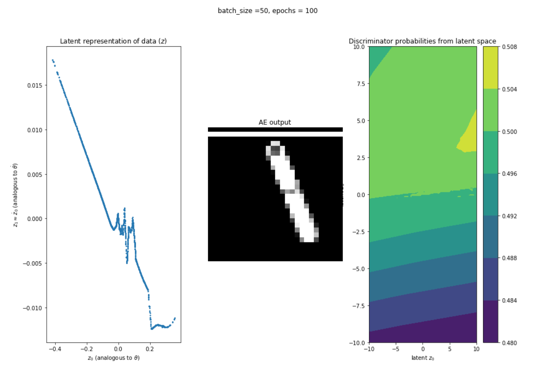
\includegraphics[width=\textwidth]{figures/gan_phase_1stack.png}
\end{subfigure}
\begin{subfigure}{0.7\textwidth}
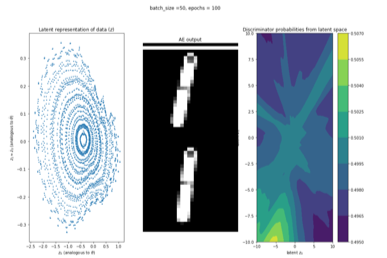
\includegraphics[width=\textwidth]{figures/gan_phase_2stack.png}
\end{subfigure}
\begin{subfigure}{0.7\textwidth}
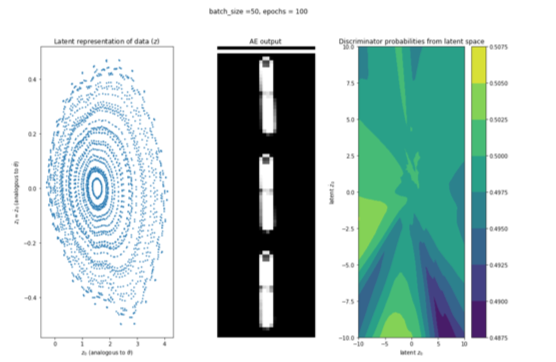
\includegraphics[width=\textwidth]{figures/gan_phase_3stack.png}
\end{subfigure}
\end{figure}

We carried out an extensive study between batch size and epoch. However, we find no consistency in the generated phase space.

\subsubsection*{key takeaways}

Preliminary results show that GANs are difficult to work with (this could be an interesting topic to cover on its own). I believe gradient clipping is one way to solve this issue. 
More importantly, Variational Integrator Networks proves that the learnt phase space from an AE will not, in general, represent the true phase space. In order to do this, one needs to encode the Lie group dynamics.
Constrained GANs have already been looked at for generating consistent results.

We still have yet to establish why a potential Lie group constrained GAN can help the world. i.e. why is it useful to be able to generate random samples of a pendulum swinging?


\subsection{VIGN}

Need to fill this section out in detail.


\subsection{Lagrangian Dynamics (WIP)}
The Euler-Lagrange formulation equates to:

$$ \frac{\partial}{\partial t} (\frac{\partial L}{\partial \dot{q}}) = \frac{\partial L}{\partial q} $$

where:
$$ L = T - U $$

In the example of a pendulum:

$$ T = 1/2 mv^2 = 1/2 m (l\dot{\theta})^2 = 1/2 m l^2 \dot{\theta}^2 $$

$$ U = mgh = mgl(1- \cos \theta) $$

$$ L = 1/2 m l^2 \dot{\theta}^2 - mgl(1-\cos\theta) $$

Placing the above into the euler-lagrange form gives us:

LHS:

$$ \frac{\partial L}{\partial \dot{q}} = ml^2 \dot{\theta}$$

$$ \frac{\partial}{\partial t} (\frac{\partial L}{\partial \dot{q}}) = ml^2 \ddot{\theta} $$

RHS:

$$ \frac{\partial L}{\partial q} = -mgl\sin\theta$$

Therefore:

$$ \ddot{\theta} = \frac{g}{l} \sin \theta $$


Now, to transition to the Hamiltonian version:

We can write the hamiltonian as the sum of the energies:

$$ H = T + U $$

$$ H = p^2/2m + U $$

$$ H = -L + 2K $$

$$ H = -L + mv^2$$

$$ H = -L + p^2/m = -L + p* (m\dot{q})/m = -L + p\dot{q}$$

$$ p = \frac{\partial L}{\partial \dot{q}} $$


\section{Running Ideas}

\subsection{VIGN extension}

- non conserved energy domain
is there a link between the port-hamiltonian view and lagrangians with generalized force
for a damped system we have:

$$ \frac{d}{dt} \frac{\partial \mathcal{L}}{\partial \dot{q}} - \frac{\partial \mathcal{L}}{\partial q} = \mathbf{F}^{ext} \frac{\partial \mathbf{r}}{\partial q}$$

see \href{http://www.physics.hmc.edu/~saeta/courses/p111/uploads/Y2013/lec131023-DSHO.pdf}{here} for details on how this equation was built. 

- distributional assumptions for practical purposes

Assume $ H = E_c $ for a trajectory of an initial condition, then:

$$ H = K + U $$

$$U = H - K $$

$$ L = K - U $$

$$ L = 2K -H $$

Now, for L to be constant, K needs to be constant. In most cases, $ K = p^2/2m $. For this to be constant p should be constant. For p to be constant, $\dot{p} = 0$. This would imply, for most settings, that:

$$ \frac{dp}{dt} = \frac{dU}{dq} = 0 $$

This means that U is zero, which is not true.

We have proven that as long as energy is conserved in a system exhibiting $K = p^2/2m$ the Lagrangian will never be constant unless the system has 0 potential. 

As such, the Lagrangian depends on the distribution of the kinetic energy/potential energy. In the large N limit, these distributions tend toward a Gaussian.

Is it beneficial to have a target variable distributed more broadly like a gaussian vs a delta?


\subsection{Covid}


SEIR model is differentiable and has some hamiltonian/energy conserving property. how might we build a neural network on this?

We start out using SEIR to model china and it works well.

We have issues modeling beijing which is seeing a second spike, we could reshape R naught (t) as an exponential sine function.
$$ R_0(t) = Ae^{-(t-t_0)}|sin(B(t-t_0))| $$

This is too specific. How can we encode the SEIR model into a graph neural network. Note, graph networks and graph neural networks are different frameworks encompassing the same core operations. In graph networks, however, the intermediate functional representations (hidden layers) are computed first, before an aggregation scheme is used. In graph neural networks, e.g. GCN, the operations involve computing a hidden layer first using neighbouring nodes, before feeding these hidden layers into the graph neural network.

This reversal means one needs to be careful in how they define graph neural network architectures between DGL and deepmind graph nets library.

We use graph convolutions to train on simulated data, we find hypersensitivity to initial conditions. More importantly, because of the time dependent nature of the system we are unsure of how many lag-variables are necessary to evolve the system.

\subsection{Inductive  biases for RL}

MDPs with policies which are deterministic or stochastic. Model free which involves sampling at random. Model based which involves sampling the learnt environment.


\bibliography{references.bib}



\end{document}
